% Options for packages loaded elsewhere
\PassOptionsToPackage{unicode}{hyperref}
\PassOptionsToPackage{hyphens}{url}
\documentclass[
  11pt,
]{article}
\usepackage{xcolor}
\usepackage[left=3cm,right=5cm,top=2cm,bottom=2cm]{geometry}
\usepackage{amsmath,amssymb}
\setcounter{secnumdepth}{5}
\usepackage{iftex}
\ifPDFTeX
  \usepackage[T1]{fontenc}
  \usepackage[utf8]{inputenc}
  \usepackage{textcomp} % provide euro and other symbols
\else % if luatex or xetex
  \usepackage{unicode-math} % this also loads fontspec
  \defaultfontfeatures{Scale=MatchLowercase}
  \defaultfontfeatures[\rmfamily]{Ligatures=TeX,Scale=1}
\fi
\usepackage{lmodern}
\ifPDFTeX\else
  % xetex/luatex font selection
\fi
% Use upquote if available, for straight quotes in verbatim environments
\IfFileExists{upquote.sty}{\usepackage{upquote}}{}
\IfFileExists{microtype.sty}{% use microtype if available
  \usepackage[]{microtype}
  \UseMicrotypeSet[protrusion]{basicmath} % disable protrusion for tt fonts
}{}
\makeatletter
\@ifundefined{KOMAClassName}{% if non-KOMA class
  \IfFileExists{parskip.sty}{%
    \usepackage{parskip}
  }{% else
    \setlength{\parindent}{0pt}
    \setlength{\parskip}{6pt plus 2pt minus 1pt}}
}{% if KOMA class
  \KOMAoptions{parskip=half}}
\makeatother
\usepackage{color}
\usepackage{fancyvrb}
\newcommand{\VerbBar}{|}
\newcommand{\VERB}{\Verb[commandchars=\\\{\}]}
\DefineVerbatimEnvironment{Highlighting}{Verbatim}{commandchars=\\\{\}}
% Add ',fontsize=\small' for more characters per line
\usepackage{framed}
\definecolor{shadecolor}{RGB}{248,248,248}
\newenvironment{Shaded}{\begin{snugshade}}{\end{snugshade}}
\newcommand{\AlertTok}[1]{\textcolor[rgb]{0.94,0.16,0.16}{#1}}
\newcommand{\AnnotationTok}[1]{\textcolor[rgb]{0.56,0.35,0.01}{\textbf{\textit{#1}}}}
\newcommand{\AttributeTok}[1]{\textcolor[rgb]{0.13,0.29,0.53}{#1}}
\newcommand{\BaseNTok}[1]{\textcolor[rgb]{0.00,0.00,0.81}{#1}}
\newcommand{\BuiltInTok}[1]{#1}
\newcommand{\CharTok}[1]{\textcolor[rgb]{0.31,0.60,0.02}{#1}}
\newcommand{\CommentTok}[1]{\textcolor[rgb]{0.56,0.35,0.01}{\textit{#1}}}
\newcommand{\CommentVarTok}[1]{\textcolor[rgb]{0.56,0.35,0.01}{\textbf{\textit{#1}}}}
\newcommand{\ConstantTok}[1]{\textcolor[rgb]{0.56,0.35,0.01}{#1}}
\newcommand{\ControlFlowTok}[1]{\textcolor[rgb]{0.13,0.29,0.53}{\textbf{#1}}}
\newcommand{\DataTypeTok}[1]{\textcolor[rgb]{0.13,0.29,0.53}{#1}}
\newcommand{\DecValTok}[1]{\textcolor[rgb]{0.00,0.00,0.81}{#1}}
\newcommand{\DocumentationTok}[1]{\textcolor[rgb]{0.56,0.35,0.01}{\textbf{\textit{#1}}}}
\newcommand{\ErrorTok}[1]{\textcolor[rgb]{0.64,0.00,0.00}{\textbf{#1}}}
\newcommand{\ExtensionTok}[1]{#1}
\newcommand{\FloatTok}[1]{\textcolor[rgb]{0.00,0.00,0.81}{#1}}
\newcommand{\FunctionTok}[1]{\textcolor[rgb]{0.13,0.29,0.53}{\textbf{#1}}}
\newcommand{\ImportTok}[1]{#1}
\newcommand{\InformationTok}[1]{\textcolor[rgb]{0.56,0.35,0.01}{\textbf{\textit{#1}}}}
\newcommand{\KeywordTok}[1]{\textcolor[rgb]{0.13,0.29,0.53}{\textbf{#1}}}
\newcommand{\NormalTok}[1]{#1}
\newcommand{\OperatorTok}[1]{\textcolor[rgb]{0.81,0.36,0.00}{\textbf{#1}}}
\newcommand{\OtherTok}[1]{\textcolor[rgb]{0.56,0.35,0.01}{#1}}
\newcommand{\PreprocessorTok}[1]{\textcolor[rgb]{0.56,0.35,0.01}{\textit{#1}}}
\newcommand{\RegionMarkerTok}[1]{#1}
\newcommand{\SpecialCharTok}[1]{\textcolor[rgb]{0.81,0.36,0.00}{\textbf{#1}}}
\newcommand{\SpecialStringTok}[1]{\textcolor[rgb]{0.31,0.60,0.02}{#1}}
\newcommand{\StringTok}[1]{\textcolor[rgb]{0.31,0.60,0.02}{#1}}
\newcommand{\VariableTok}[1]{\textcolor[rgb]{0.00,0.00,0.00}{#1}}
\newcommand{\VerbatimStringTok}[1]{\textcolor[rgb]{0.31,0.60,0.02}{#1}}
\newcommand{\WarningTok}[1]{\textcolor[rgb]{0.56,0.35,0.01}{\textbf{\textit{#1}}}}
\usepackage{longtable,booktabs,array}
\newcounter{none} % for unnumbered tables
\usepackage{calc} % for calculating minipage widths
% Correct order of tables after \paragraph or \subparagraph
\usepackage{etoolbox}
\makeatletter
\patchcmd\longtable{\par}{\if@noskipsec\mbox{}\fi\par}{}{}
\makeatother
% Allow footnotes in longtable head/foot
\IfFileExists{footnotehyper.sty}{\usepackage{footnotehyper}}{\usepackage{footnote}}
\makesavenoteenv{longtable}
\usepackage{graphicx}
\makeatletter
\newsavebox\pandoc@box
\newcommand*\pandocbounded[1]{% scales image to fit in text height/width
  \sbox\pandoc@box{#1}%
  \Gscale@div\@tempa{\textheight}{\dimexpr\ht\pandoc@box+\dp\pandoc@box\relax}%
  \Gscale@div\@tempb{\linewidth}{\wd\pandoc@box}%
  \ifdim\@tempb\p@<\@tempa\p@\let\@tempa\@tempb\fi% select the smaller of both
  \ifdim\@tempa\p@<\p@\scalebox{\@tempa}{\usebox\pandoc@box}%
  \else\usebox{\pandoc@box}%
  \fi%
}
% Set default figure placement to htbp
\def\fps@figure{htbp}
\makeatother
% definitions for citeproc citations
\NewDocumentCommand\citeproctext{}{}
\NewDocumentCommand\citeproc{mm}{%
  \begingroup\def\citeproctext{#2}\cite{#1}\endgroup}
\makeatletter
 % allow citations to break across lines
 \let\@cite@ofmt\@firstofone
 % avoid brackets around text for \cite:
 \def\@biblabel#1{}
 \def\@cite#1#2{{#1\if@tempswa , #2\fi}}
\makeatother
\newlength{\cslhangindent}
\setlength{\cslhangindent}{1.5em}
\newlength{\csllabelwidth}
\setlength{\csllabelwidth}{3em}
\newenvironment{CSLReferences}[2] % #1 hanging-indent, #2 entry-spacing
 {\begin{list}{}{%
  \setlength{\itemindent}{0pt}
  \setlength{\leftmargin}{0pt}
  \setlength{\parsep}{0pt}
  % turn on hanging indent if param 1 is 1
  \ifodd #1
   \setlength{\leftmargin}{\cslhangindent}
   \setlength{\itemindent}{-1\cslhangindent}
  \fi
  % set entry spacing
  \setlength{\itemsep}{#2\baselineskip}}}
 {\end{list}}
\usepackage{calc}
\newcommand{\CSLBlock}[1]{\hfill\break\parbox[t]{\linewidth}{\strut\ignorespaces#1\strut}}
\newcommand{\CSLLeftMargin}[1]{\parbox[t]{\csllabelwidth}{\strut#1\strut}}
\newcommand{\CSLRightInline}[1]{\parbox[t]{\linewidth - \csllabelwidth}{\strut#1\strut}}
\newcommand{\CSLIndent}[1]{\hspace{\cslhangindent}#1}
\setlength{\emergencystretch}{3em} % prevent overfull lines
\providecommand{\tightlist}{%
  \setlength{\itemsep}{0pt}\setlength{\parskip}{0pt}}
\usepackage{amsmath,amsfonts,amssymb}
\usepackage{booktabs}
\usepackage{float}
\DeclareMathOperator{\Var}{Var}
\DeclareMathOperator{\Cov}{Cov}
\DeclareMathOperator{\tr}{tr}
\usepackage{bookmark}
\IfFileExists{xurl.sty}{\usepackage{xurl}}{} % add URL line breaks if available
\urlstyle{same}
\hypersetup{
  pdftitle={Power Analysis for Longitudinal Clinical Trials with Run-In and Common Close Observations},
  pdfauthor={Ronald G. Thomas},
  hidelinks,
  pdfcreator={LaTeX via pandoc}}

\title{Power Analysis for Longitudinal Clinical Trials with Run-In and
Common Close Observations}
\author{Ronald G. Thomas}
\date{May 08, 2026}

\begin{document}
\maketitle
\begin{abstract}
\textbf{Background.} Longitudinal clinical trials often incorporate
pre-randomisation (run-in) and post-treatment (common close)
observations to improve estimator efficiency. Closed-form power and
sample-size formulas for these augmented designs under linear
mixed-effects models with random slopes have remained scattered across
the literature and partially specified, making applied sample-size
calculation cumbersome.

\textbf{Methods.} We derive closed-form power and sample-size formulas
for three nested cases: (i) two run-in observations, (ii) an arbitrary
number \(J_0\) of run-in observations, and (iii) \(J_0\) run-in plus
\(J_2\) common close observations. All derivations proceed via the
Woodbury matrix identity applied to the GLS estimator under change-score
parameterisation. The formulas are expressed in terms of the residual
variance \(\sigma^2\), the random-slope variance \(\sigma_b^2\), and the
observation spacing \(t\), enabling direct computation of required
sample sizes.

\textbf{Results.} Numerical examples using parameters from Alzheimer's
disease neuroimaging trials demonstrate that two run-in observations can
reduce required sample sizes by 30-45\%, with additional gains from
common close observations. The closed-form expressions allow sensitivity
analysis with respect to the signal-to-noise ratio \(\sigma_b / \sigma\)
without re-running simulation.

\textbf{Conclusions.} The Woodbury-based formulas are the simplest
available closed-form expressions for the variance of the
treatment-effect estimator under random-slopes longitudinal-trial
designs with run-in and common close observations. They serve as a
foundation for the AR(1) extension (Paper 2), the optimal-allocation
problem (Paper 3), and the GLS-versus-ANCOVA-versus-averaged estimator
comparison (Paper 4) in this compendium.
\end{abstract}

{
\setcounter{tocdepth}{2}
\tableofcontents
}
\section{Introduction}\label{introduction}

The run-in period has served multiple purposes in clinical trial design,
from identifying compliant participants to washing out prior treatments
(\citeproc{ref-packerWhyHasRunIn2017}{Packer 2017}). A distinct and
methodologically important use has emerged in trials where the primary
outcome is a rate of change: estimating individual baseline trajectories
that, when incorporated into the analysis model, substantially increase
statistical power.

Frost et al. (\citeproc{ref-frostOptimizingDesignClinical2008}{2008})
established the theoretical foundation for this approach within the
linear mixed effects framework. Their key insight was that when
between-subject variability in rates of change is large relative to
measurement error, pre-randomization observations provide valuable
information about each participant's underlying trajectory, reducing the
residual variance of the treatment effect estimator. Working with
neuroimaging outcomes in Alzheimer's disease trials, where the ratio of
slope variability to measurement error is particularly favorable, they
demonstrated sample size reductions of 30--45\%.

Wang et al. (\citeproc{ref-wangTwoPeriodLinear2019}{2019}) extended this
framework by proposing two-period linear mixed effects models that
jointly model run-in and post-randomization data rather than using
run-in observations merely as covariates. Their approach yields
additional power gains of up to 15\% and enables unequal randomization
ratios without power loss, since run-in observations effectively
contribute placebo-equivalent information for all participants.

A parallel literature has developed closed-form variance and sample size
formulae for the random coefficient regression model without a run-in
phase. Lu et al. (\citeproc{ref-lu2009}{2009}) derived the variance of
the constrained longitudinal data analysis estimator and its relation to
analysis of covariance, and Lu (\citeproc{ref-lu2010}{2010}) established
efficiency conditions under which the two approaches coincide. Hu et al.
(\citeproc{ref-hu2021}{2021}) generalized these results to random
coefficient regression models with monotone missing data and variable
follow-up, providing variance, power, and sample size expressions
illustrated with data from the Alzheimer's Disease Neuroimaging
Initiative. These formulae apply to designs with \(J_0 = 0\) run-in
observations and an arbitrary post-randomization visit schedule, and
serve as the baseline case that the present paper extends.

The CRAN reference implementation of the \(J_0=0\) formulae is the
\texttt{longpower} package (\citeproc{ref-iddi2022}{Iddi and Donohue
2022}), which provides the routines \texttt{edland.linear.power()},
\texttt{diggle.linear.power()}, and \texttt{liu.liang.linear.power()}
for slope-comparison trials with random intercepts and slopes
(\citeproc{ref-ard2011}{Ard and Edland 2011};
\citeproc{ref-diggle2002}{Diggle et al. 2002};
\citeproc{ref-liuliang1997}{Liu and Liang 1997}). We show in Section 3.3
that the closed-form result derived below reduces to the Ard-Edland
slope-variance formula implemented in \texttt{edland.linear.power()} at
the boundary \(J_0 = J_2 = 0\), and to the Diggle compound-symmetry
formula when additionally \(\sigma_b^2 = 0\). The generalization
developed here therefore embeds the existing \texttt{longpower} formulae
as the baseline case against which the efficiency gains from run-in and
common close observations are measured.

Despite these advances, no general closed-form power formula has been
derived that simultaneously accounts for an arbitrary number of run-in
observations and a separate set of common close observations collected
after treatment cessation. The common close phase, in which all
participants are observed off-treatment following the randomized period,
provides additional information about individual trajectories at no cost
to the treatment comparison. Post-treatment observation periods appear
in delayed-start and randomized withdrawal designs aimed at
distinguishing symptomatic from disease-modifying effects
(\citeproc{ref-sperlingA4StudyStopping2014}{Sperling et al. 2014}), but
the contribution of the common close to statistical efficiency within
the GLS framework has not been formally characterized.

This paper presents three results. First, we derive a simple closed-form
variance formula for the treatment effect estimator when exactly two
run-in observations precede randomization (Section 3.2). Second, we
generalize this formula to an arbitrary number \(J_0\) of run-in
observations (Section 3.3). Third, we further extend to include \(J_2\)
common close observations collected after treatment cessation (Section
3.4). All derivations proceed from the generalized least squares
estimator under the Woodbury matrix identity, yielding expressions in
terms of the residual variance \(\sigma^2\), the random slope variance
\(\sigma_b^2\), and the observation spacing \(t\). Section 5 provides
numerical examples using parameters estimated from Alzheimer's disease
neuroimaging studies.

\section{Model}\label{model}

\subsection{General formulation}\label{general-formulation}

Consider a two-arm longitudinal clinical trial in which \(N\)
participants are observed at equally spaced time points across three
phases: a run-in period (pre-randomization), a treatment period
(post-randomization), and an optional common close period
(post-treatment). Let \(Y_{ij}\) denote the outcome for participant
\(i\) at time point \(j\). The observation schedule is:

\begin{itemize}
\tightlist
\item
  \textbf{Run-in:} \(j = -J_0, -J_0+1, \ldots, -1\) (all participants
  untreated)
\item
  \textbf{Randomization visit:} \(j = 0\) (baseline)
\item
  \textbf{Treatment period:} \(j = 1, 2, \ldots, J_1\) (participants
  randomized to treatment or placebo)
\item
  \textbf{Common close:} \(j = J_1+1, J_1+2, \ldots, J_1+J_2\) (all
  participants off-treatment)
\end{itemize}

We model the outcome as \begin{equation}
  Y_{ij} = \alpha + a_i +
  \bigl(\delta(1-h_j) + \beta h_j + \gamma h_j g_i + b_i
  \bigr) t_j + e_{ij}
  \label{eq:model}
\end{equation} where \(\alpha\) is the overall intercept,
\(a_i \sim N(0,
\sigma_a^2)\) is a random intercept, \(b_i \sim N(0,
\sigma_b^2)\) is a random slope, and \(e_{ij} \sim N(0,
\sigma^2)\) are independent residual errors. The phase indicator is \[
  h_j =
  \begin{cases}
    0 & \text{if } j \le 0 \quad \text{(run-in)} \\
    1 & \text{if } j > 0 \quad \text{(post-randomization)}
  \end{cases}
\] and the treatment group indicator is \[
  g_i =
  \begin{cases}
    1 & i = 1, \ldots, m
      \quad \text{(treatment)} \\
    0 & i = m+1, \ldots, N
      \quad \text{(placebo)}
  \end{cases}
\]

The fixed effects are: \(\delta\), the rate of change during the run-in
period (common to all participants); \(\beta\), the rate of change
during the post-randomization period for the placebo group; and
\(\gamma\), the treatment effect on the rate of change. We assume
equally spaced observations with interval \(t\), so \(t_j = jt\).

For the common close phase (\(j > J_1\)), both treatment and placebo
groups revert to a common off-treatment slope. We model this by setting
\(g_i = 0\) for all participants during the common close, so that the
slope for both groups is \(\beta
+ b_i\) in this phase. This is equivalent to replacing the treatment
indicator with \(g_i \cdot I(1 \le j \le J_1)\) in model
\eqref{eq:model}.

\subsection{Change-score
parameterization}\label{change-score-parameterization}

Following Frost et al.
(\citeproc{ref-frostOptimizingDesignClinical2008}{2008}), we work with
change scores relative to the randomization visit: \begin{equation}
  c_{ij} = Y_{ij} - Y_{i0}
  \label{eq:change}
\end{equation}

This eliminates the intercept \(\alpha\) and the random intercept
\(a_i\). We note that the change-score approach is algebraically
equivalent to constrained longitudinal data analysis (cLDA) under
compound symmetry, where the baseline is included in the response vector
with a common-mean constraint across treatment groups
(\citeproc{ref-lairdlRandomEffectsModelsLongitudinal2023}{Lairdl and
Warel 2023};
\citeproc{ref-wangProportionalConstrainedLongitudinal2022}{Wang et al.
2022}). The variance formulas derived below therefore apply to both
change-score and cLDA analyses of run-in designs. Because the
change-score eliminates \(a_i\), the resulting formulas depend on only
two variance components (\(\sigma^2, \sigma_b^2\)) rather than the three
(\(\sigma^2, \sigma_a^2, \sigma_b^2\)) required by the raw-outcome
model. Zhao and Edland (\citeproc{ref-Zhao2021}{2021}) show that
ignoring the intercept-slope correlation in the three-component model
can produce anticonservative sample sizes; the change-score approach
avoids this issue by construction, at the cost of discarding information
about \(\sigma_a^2\). The change-score formulation yields
\begin{equation}
  c_{ij} = \bigl(\delta(1-h_j) + \beta h_j
    + \gamma h_j g_i + b_i\bigr) t_j
    + (e_{ij} - e_{i0})
  \label{eq:change_model}
\end{equation} for \(j \ne 0\). The change-score vector for participant
\(i\) has dimension \(J = J_0 + J_1 + J_2\), encompassing all three
phases.

\subsection{Covariance structure}\label{covariance-structure}

The marginal covariance of the change-score vector is \begin{equation}
  \Sigma = R + Z G Z'
  \label{eq:sigma}
\end{equation} where \(G = \sigma_b^2\) (scalar, since we have a single
random slope), \(Z = t \cdot \mathbf{1}_J\) is the \(J \times 1\) random
effects design vector, and \(R\) is the \(J \times J\) residual
covariance of the differenced errors \((e_{ij} - e_{i0})\).

The residual covariance has the structure \begin{equation}
  R_{jl} = \mathop{\mathrm{Cov}}(e_{ij} - e_{i0},\; e_{il} - e_{i0})
  = \begin{cases}
    2\sigma^2 & \text{if } j = l \\
    \sigma^2  & \text{if } j \ne l
  \end{cases}
  \label{eq:R}
\end{equation} since \(e_{ij}\) are independent with common variance
\(\sigma^2\), and the baseline error \(e_{i0}\) induces positive
correlation among all change scores. Thus
\(R = \sigma^2(\mathbf{I}_J + \mathbf{1}_J \mathbf{1}_J')\).

\section{Variance of the Treatment Effect
Estimator}\label{variance-of-the-treatment-effect-estimator}

\subsection{GLS estimation and the Woodbury
identity}\label{gls-estimation-and-the-woodbury-identity}

The generalized least squares estimator of the fixed effects is
\begin{equation}
  \hat{\boldsymbol{\beta}} = (X' \Sigma^{-1} X)^{-1} X' \Sigma^{-1}
  \mathbf{c}
  \label{eq:gls}
\end{equation} with
\(\mathop{\mathrm{Var}}(\hat{\boldsymbol{\beta}}) = (X' \Sigma^{-1} X)^{-1}\),
where \(X\) is the fixed effects design matrix and \(\mathbf{c}\) is the
stacked change-score vector. Our target is
\(\mathop{\mathrm{Var}}(\hat{\gamma})\), the variance of the treatment
effect estimator, which is the diagonal element of
\((X' \Sigma^{-1} X)^{-1}\) corresponding to \(\gamma\).

The key computational tool is the Woodbury matrix identity. Since
\(\Sigma = R + Z G Z'\) with scalar \(G = \sigma_b^2\): \begin{equation}
  \Sigma^{-1} = R^{-1} - R^{-1} Z
    \bigl(G^{-1} + Z' R^{-1} Z\bigr)^{-1}
    Z' R^{-1}
  \label{eq:woodbury}
\end{equation}

This avoids direct inversion of the \(J \times J\) matrix \(\Sigma\) and
enables closed-form results because \(R^{-1}\) has a known simple
structure.

From \(R = \sigma^2(\mathbf{I}_J + \mathbf{1}_J
\mathbf{1}_J')\), the Sherman-Morrison formula gives \begin{equation}
  R^{-1} = \frac{1}{\sigma^2}\left(
    \mathbf{I}_J - \frac{1}{J+1}
    \mathbf{1}_J \mathbf{1}_J'
  \right)
  \label{eq:Rinv}
\end{equation}

With \(Z = t \cdot \mathbf{1}_J\), we obtain \begin{equation}
  Z' R^{-1} Z = \frac{t^2}{\sigma^2}
    \left(J - \frac{J^2}{J+1}\right)
  = \frac{J\, t^2}{\sigma^2(J+1)}
  \label{eq:ZRZ}
\end{equation} and \begin{equation}
  \bigl(G^{-1} + Z' R^{-1} Z\bigr)^{-1}
  = \frac{\sigma^2 \sigma_b^2 (J+1)}
    {\sigma^2(J+1) + J\, t^2 \sigma_b^2}
  \label{eq:H}
\end{equation}

Let \(a = \sigma^2\) and \(b = \sigma_b^2\) for conciseness. Define
\begin{equation}
  \eta_J = \frac{a(J+1) + J\, t^2 b}{a(J+1)}
  = 1 + \frac{J\, t^2 b}{a(J+1)}
  \label{eq:eta}
\end{equation} so that \((G^{-1} + Z'R^{-1}Z)^{-1} = b / \eta_J\).

\subsubsection{Per-participant information, compact
form}\label{per-participant-information-compact-form}

Let \(X_i\), \(Z_i\), and \(R_i\) denote the per-participant fixed
effects design, random effects design, and residual covariance, and
define the scalar \begin{equation}
  \mathcal{J}_i
  = Z_i' R_i^{-1} Z_i + G^{-1}
  \label{eq:Ji}
\end{equation} By (\ref{eq:woodbury}), the per-participant contribution
to the GLS information matrix is \begin{equation}
  X_i' \Sigma_i^{-1} X_i
  = X_i' R_i^{-1} X_i
    - \frac{(X_i' R_i^{-1} Z_i)(Z_i' R_i^{-1} X_i)}
           {\mathcal{J}_i}
  \label{eq:perpt_info}
\end{equation} and the total information is \(X' \Sigma^{-1} X = \sum_i
X_i' \Sigma_i^{-1} X_i\), with
\(\mathop{\mathrm{Var}}(\hat{\boldsymbol{\beta}})
= (X' \Sigma^{-1} X)^{-1}\). Two features of this form are used later:
(i) under a single random slope, \(\mathcal{J}_i\) is a scalar so
(\ref{eq:perpt_info}) is a rank-one correction of the OLS-style
information \(X_i' R_i^{-1} X_i\); (ii) because per-participant
contributions add, heterogeneous designs (varying \(J_0\), \(J_2\), or
dropout patterns) are accommodated by summing (\ref{eq:perpt_info}) over
the relevant strata.

\subsection{\texorpdfstring{Case 1: Standard design, no run-in
(\(J_0=0\), \(J_1=2\),
\(J_2=0\))}{Case 1: Standard design, no run-in (J\_0=0, J\_1=2, J\_2=0)}}\label{case-1-standard-design-no-run-in-j_00-j_12-j_20}

This case reproduces the result in Frost et al.
(\citeproc{ref-frostOptimizingDesignClinical2008}{2008}), Section 3.1.1,
and is the \(J_0 = 0\) baseline of the random coefficient regression
power formulae of Lu et al. (\citeproc{ref-lu2009}{2009}) and Hu et al.
(\citeproc{ref-hu2021}{2021}). It serves as verification for our
framework.

With \(J_0=0\) and \(J_1=2\), there are \(J = 2\) change scores
\((c_{i,1},\, c_{i,2})\) at post-randomization times \((t,\,
2t)\). Since there is no run-in, the model has two fixed effects: the
placebo slope \(\beta\) and the treatment effect \(\gamma\). The design
matrices are: \[
  X_i^{(\text{trt})} = t\begin{pmatrix}
    1 & 1 \\ 2 & 2
  \end{pmatrix}, \qquad
  X_i^{(\text{plc})} = t\begin{pmatrix}
    1 & 0 \\ 2 & 0
  \end{pmatrix}
\]

The residual covariance is
\(R = a \begin{pmatrix} 2 & 1 \\ 1 & 2 \end{pmatrix}\) with
\(R^{-1} = \frac{1}{3a}
\begin{pmatrix} 2 & -1 \\ -1 & 2 \end{pmatrix}\), and the random effects
design is \(Z = t(1,\, 2)'\).

Applying the Woodbury identity with \(J = 2\): \begin{equation}
  Z'R^{-1}Z = \frac{t^2}{3a}(1,\,2)
    \begin{pmatrix}2&-1\\-1&2\end{pmatrix}
    \begin{pmatrix}1\\2\end{pmatrix}
  = \frac{t^2}{3a}(1,\,2)(0,\,3)' = \frac{6t^2}{3a}
  = \frac{2t^2}{a}
\end{equation} \begin{equation}
  (G^{-1} + Z'R^{-1}Z)^{-1}
  = \frac{ab}{a + 2bt^2}
\end{equation}

After summing over one treatment and one placebo participant, the
information matrix is \begin{equation}
  X'\Sigma^{-1}X
  = \frac{2t^2}{a + 2bt^2}
    \begin{pmatrix} 2 & 1 \\ 1 & 1 \end{pmatrix}
\end{equation} and its inverse is \begin{equation}
  \mathop{\mathrm{Var}}(\hat{\boldsymbol{\beta}})
  = \frac{a + 2bt^2}{2t^2}
    \begin{pmatrix} 1 & -1 \\ -1 & 2 \end{pmatrix}
  \label{eq:var_frost}
\end{equation}

The variance of the treatment effect estimator (per participant pair) is
the \((2,2)\) element: \begin{equation}
  \boxed{
    \mathop{\mathrm{Var}}(\hat{\gamma})\big|_{J_0=0,J_1=2}
    = \frac{a + 2bt^2}{t^2}
    = \frac{\sigma^2 + 2\sigma_b^2 t^2}{t^2}
  }
  \label{eq:var_r0k2}
\end{equation}

This agrees with Frost et al.~(2008), Section 3.1.1. For \(m\)
participants per group:
\(\mathop{\mathrm{Var}}(\hat{\gamma}) = (\sigma^2 + 2\sigma_b^2 t^2) /
(m t^2)\). This serves as the baseline against which the run-in designs
are compared.

\subsection{\texorpdfstring{Case 2: Two run-in observations (\(J_0=2\),
\(J_1=1\),
\(J_2=0\))}{Case 2: Two run-in observations (J\_0=2, J\_1=1, J\_2=0)}}\label{case-2-two-run-in-observations-j_02-j_11-j_20}

We now have \(J = 3\) change scores \((c_{i,-2},\, c_{i,-1},\,
c_{i,1})\) at times \((-2t,\, -t,\, 0,\, t)\). The fixed effects design
matrix separates the run-in slope \(\delta\) from the post-randomization
slopes: \[
  X_i^{(\text{trt})} = \begin{pmatrix}
    -2t & 0 & 0 \\ -t & 0 & 0 \\ 0 & t & t
  \end{pmatrix}, \qquad
  X_i^{(\text{plc})} = \begin{pmatrix}
    -2t & 0 & 0 \\ -t & 0 & 0 \\ 0 & t & 0
  \end{pmatrix}
\]

The random effects design is \(Z = t(1,\, 1,\, 1)' \cdot
(-2,\, -1,\, 1)' \cdot b_i\). However, since the random slope applies
uniformly to all time points, \(Z = t(-2,\, -1,
\, 1)'\) for the random effect \(b_i\). We note that the change scores
at times \(-2t\) and \(-t\) relative to baseline at \(0\) yield
\(c_{i,-2} = Y_{i,-2} - Y_{i,0}\) and \(c_{i,-1} = Y_{i,-1} - Y_{i,0}\).

More carefully, under model \eqref{eq:model}: \begin{align}
  c_{i,-2} &= -2(\delta + b_i)\,t + (e_{i,-2} - e_{i,0})
    \notag \\
  c_{i,-1} &= -(\delta + b_i)\,t + (e_{i,-1} - e_{i,0})
    \notag \\
  c_{i,1}  &= (\beta + \gamma g_i + b_i)\,t
    + (e_{i,1} - e_{i,0})
  \label{eq:c_r2}
\end{align}

Thus the design matrices for the fixed effects
\((\delta,\, \beta,\, \gamma)'\) are: \[
  X_i^{(\text{trt})} = t\begin{pmatrix}
    -2 & 0 & 0 \\ -1 & 0 & 0 \\ 0 & 1 & 1
  \end{pmatrix}, \qquad
  X_i^{(\text{plc})} = t\begin{pmatrix}
    -2 & 0 & 0 \\ -1 & 0 & 0 \\ 0 & 1 & 0
  \end{pmatrix}
\] and the random effects design is \(Z_i = t(-2,\, -1,\, 1)'\).

The residual covariance is \begin{equation}
  R = a\begin{pmatrix}
    2 & 1 & 1 \\ 1 & 2 & 1 \\ 1 & 1 & 2
  \end{pmatrix}
  = a(\mathbf{I}_3 + \mathbf{1}_3\mathbf{1}_3')
\end{equation} with inverse \begin{equation}
  R^{-1} = \frac{1}{a}\left(\mathbf{I}_3
    - \frac{1}{4}\mathbf{1}_3\mathbf{1}_3'\right)
  = \frac{1}{4a}\begin{pmatrix}
    3 & -1 & -1 \\ -1 & 3 & -1 \\ -1 & -1 & 3
  \end{pmatrix}
\end{equation}

Now we compute the Woodbury components. With \(Z = t(-2,\, -1,\, 1)'\):
\begin{equation}
  Z'R^{-1}Z = \frac{t^2}{4a}\bigl(
    3 \cdot 4 + 3 \cdot 1 + 3 \cdot 1
    - 2(-1)(-2)(-1) - 2(-1)(-2)(1)
    - 2(-1)(-1)(1)\bigr)
\end{equation}

Computing directly: \(Z'R^{-1}Z = \frac{t^2}{4a}(-2,\,-1,\,1)
\begin{pmatrix} 3&-1&-1 \\ -1&3&-1 \\ -1&-1&3
\end{pmatrix}
(-2,\,-1,\,1)'\)

\begin{align}
  R^{-1}Z &= \frac{t}{4a}\begin{pmatrix}
    3(-2)+(-1)(-1)+(-1)(1) \\
    (-1)(-2)+3(-1)+(-1)(1) \\
    (-1)(-2)+(-1)(-1)+3(1)
  \end{pmatrix}
  = \frac{t}{4a}\begin{pmatrix}
    -6 \\ -2 \\ 6
  \end{pmatrix}
  \notag
\end{align} so \(Z'R^{-1}Z = \frac{t^2}{4a}
[(-2)(-6)+(-1)(-2)+(1)(6)] = \frac{t^2}{4a}(12+2+6)
= \frac{20t^2}{4a} = \frac{5t^2}{a}\).

Alternatively, we note \(Z = t \cdot \mathbf{d}\) where
\(\mathbf{d} = (-2,-1,1)'\), so \(Z'R^{-1}Z =
\frac{t^2}{a}(\mathbf{d}'\mathbf{d} -
\frac{1}{4}(\mathbf{1}'\mathbf{d})^2) =
\frac{t^2}{a}(6 - \frac{4}{4}) = \frac{5t^2}{a}\).

Thus \begin{equation}
  H \equiv (G^{-1}+Z'R^{-1}Z)^{-1}
  = \frac{ab}{a + 5bt^2}
\end{equation}

For the information matrix, we compute \(X'R^{-1}X\) summed over
treatment and placebo groups. For a single treatment participant: \[
  X_i^{(\text{trt})\prime} R^{-1} X_i^{(\text{trt})}
  = \frac{t^2}{4a}\begin{pmatrix}
    -2 & -1 & 0 \\ 0 & 0 & 1 \\ 0 & 0 & 1
  \end{pmatrix}
  \begin{pmatrix}
    3&-1&-1\\-1&3&-1\\-1&-1&3
  \end{pmatrix}
  \begin{pmatrix}
    -2&0&0\\-1&0&0\\0&1&1
  \end{pmatrix}
\]

Computing the product: \begin{equation}
  X_i^{(\text{trt})\prime} R^{-1} X_i^{(\text{trt})}
  = \frac{t^2}{4a}\begin{pmatrix}
    11 & 3 & 3 \\ 3 & 3 & 3 \\ 3 & 3 & 3
  \end{pmatrix}
\end{equation}

For placebo (whose \(\gamma\) column is zero): \begin{equation}
  X_i^{(\text{plc})\prime} R^{-1} X_i^{(\text{plc})}
  = \frac{t^2}{4a}\begin{pmatrix}
    11 & 3 & 0 \\ 3 & 3 & 0 \\ 0 & 0 & 0
  \end{pmatrix}
\end{equation}

Summing (one participant per group for the derivation, then multiplying
by \(m\)): \begin{equation}
  X'R^{-1}X = \frac{t^2}{4a}\begin{pmatrix}
    22 & 6 & 3 \\ 6 & 6 & 3 \\ 3 & 3 & 3
  \end{pmatrix}
\end{equation}

For the Woodbury correction, we need \(X'R^{-1}Z\). For treatment: \[
  X_i^{(\text{trt})\prime}R^{-1}Z
  = \frac{t^2}{4a}\begin{pmatrix}-2&-1&0\\0&0&1\\0&0&1
  \end{pmatrix}
  \begin{pmatrix}-6\\-2\\6\end{pmatrix}
  = \frac{t^2}{4a}\begin{pmatrix}14\\6\\6\end{pmatrix}
\]

For placebo: \[
  X_i^{(\text{plc})\prime}R^{-1}Z
  = \frac{t^2}{4a}\begin{pmatrix}-2&-1&0\\0&0&1\\0&0&0
  \end{pmatrix}
  \begin{pmatrix}-6\\-2\\6\end{pmatrix}
  = \frac{t^2}{4a}\begin{pmatrix}14\\6\\0\end{pmatrix}
\]

The Woodbury correction requires the per-subject outer products (not the
outer product of the sum): \begin{align}
  W &= \sum_{g} X_i^{(g)\prime} R^{-1} Z
    \cdot H \cdot
    Z' R^{-1} X_i^{(g)} \notag \\
  &= \frac{bt^4}{16a(a+5bt^2)}
    \left(
      \begin{pmatrix}14\\6\\6\end{pmatrix}
      (14,6,6)
      + \begin{pmatrix}14\\6\\0\end{pmatrix}
      (14,6,0)
    \right) \notag \\
  &= \frac{bt^4}{16a(a+5bt^2)}
    \begin{pmatrix}
      392 & 168 & 84 \\
      168 & 72 & 36 \\
      84 & 36 & 36
    \end{pmatrix}
\end{align}

Therefore \begin{equation}
  X'\Sigma^{-1}X = X'R^{-1}X - W
\end{equation}

To find \(\mathop{\mathrm{Var}}(\hat{\gamma})\), we need the \((3,3)\)
element of \((X'\Sigma^{-1}X)^{-1}\). We compute this numerically in the
R code below and verify against the closed-form result.

Carrying through the algebra, define \(D = a + 5bt^2 =
\sigma^2 + 5\sigma_b^2 t^2\). The \((3,3)\) cofactor of
\(X'\Sigma^{-1}X\) simplifies to \(1536aD \cdot
t^4/(16aD)^2 = 6t^4/(16aD)\), and the determinant yields
\(\det = 16aD(3a+2bt^2)^2 \cdot t^6/(16aD)^3\). The ratio gives:

\begin{equation}
  \boxed{
    \mathop{\mathrm{Var}}(\hat{\gamma})\big|_{J_0=2,J_1=1}
    = \frac{8\sigma^2(\sigma^2 + 5\sigma_b^2 t^2)}
           {3t^2(\sigma^2 + 2\sigma_b^2 t^2)}
  }
  \label{eq:var_r2k1}
\end{equation}

Unlike the Frost formula \eqref{eq:var_r0k2}, the run-in variance
depends on \(\sigma^2\) both in the numerator and denominator,
reflecting the additional information extracted from pre-randomization
observations.

\subsection{\texorpdfstring{General formula: \(J_0\) run-in observations
(\(J_2=0\))}{General formula: J\_0 run-in observations (J\_2=0)}}\label{general-formula-j_0-run-in-observations-j_20}

We now derive the variance for arbitrary \(J_0\) run-in observations
with \(J_1\) post-randomization observations and no common close
(\(J_2 = 0\)). The total number of change scores is \(J = J_0 + J_1\).

The change scores are \begin{align}
  c_{i,-s} &= -s(\delta + b_i)\,t + (e_{i,-s} - e_{i0})
    & s &= 1,\ldots,J_0 \notag \\
  c_{i,l}  &= l(\beta + \gamma g_i + b_i)\,t
    + (e_{i,l} - e_{i0})
    & l &= 1,\ldots,J_1
\end{align}

The fixed effects design matrix has columns for
\((\delta, \beta, \gamma)\). Let \(\mathbf{d}_{J_0} = (-J_0, -J_0+1,
\ldots, -1)' \cdot t\) be the run-in time vector and
\(\mathbf{d}_{J_1} = (1, 2, \ldots, J_1)' \cdot t\) be the
post-randomization time vector. Then: \[
  X_i^{(\text{trt})} = \begin{pmatrix}
    \mathbf{d}_{J_0} & \mathbf{0} & \mathbf{0} \\
    \mathbf{0}   & \mathbf{d}_{J_1} & \mathbf{d}_{J_1}
  \end{pmatrix}, \qquad
  X_i^{(\text{plc})} = \begin{pmatrix}
    \mathbf{d}_{J_0} & \mathbf{0} & \mathbf{0} \\
    \mathbf{0}   & \mathbf{d}_{J_1} & \mathbf{0}
  \end{pmatrix}
\]

The random effects design vector is
\(Z_i = (\mathbf{d}_{J_0}',\, \mathbf{d}_{J_1}')'\), i.e., the full
vector of time distances from baseline.

The residual covariance remains \(R = a(\mathbf{I}_J +
\mathbf{1}_J\mathbf{1}_J')\) with inverse given by \eqref{eq:Rinv}.

\subsubsection{\texorpdfstring{Computing
\(X'\Sigma^{-1}X\)}{Computing X\textquotesingle\textbackslash Sigma\^{}\{-1\}X}}\label{computing-xsigma-1x}

We proceed through the Woodbury identity. Define
\(S_{J_0} = \sum_{s=1}^{J_0} s^2 = J_0(J_0+1)(2J_0+1)/6\) and
\(S_{J_1} = \sum_{l=1}^{J_1} l^2 = J_1(J_1+1)(2J_1+1)/6\).

The key intermediate quantities are:

\textbf{\(Z'R^{-1}Z\):} With \(Z = t \cdot \mathbf{d}\) where
\(\mathbf{d} = (-J_0,\ldots,-1,1,\ldots,J_1)'\): \begin{equation}
  Z'R^{-1}Z = \frac{t^2}{a}\left[
    (S_{J_0} + S_{J_1})
    - \frac{(\sum d_j)^2}{J+1}
  \right]
  \label{eq:ZRZ_general}
\end{equation} where \(\sum d_j = -J_0(J_0+1)/2 + J_1(J_1+1)/2\).

\textbf{\((G^{-1} + Z'R^{-1}Z)^{-1}\):} From \eqref{eq:ZRZ_general}: \[
  H = \frac{ab}{a + t^2 b \cdot Z'R^{-1}Z \cdot a/t^2}
\]

\textbf{\(X'R^{-1}X\):} This \(3 \times 3\) matrix has elements computed
from the block structure of \(X\). Letting
\(D_{J_0} = \sum_{s=1}^{J_0} s = J_0(J_0+1)/2\) and
\(D_{J_1} = \sum_{l=1}^{J_1} l = J_1(J_1+1)/2\), and using
\(R^{-1} = \frac{1}{a}(\mathbf{I}_J -
\frac{1}{J+1}\mathbf{1}\mathbf{1}')\), the information matrix summed
over one treatment and one placebo participant is:

\begin{equation}
  X'R^{-1}X = \frac{t^2}{a}\begin{pmatrix}
    2\!\left(S_{J_0} - \frac{D_{J_0}^2}{J+1}\right) &
    \frac{2D_{J_0} D_{J_1}}{J+1} &
    \frac{D_{J_0} D_{J_1}}{J+1} \\[4pt]
    \frac{2D_{J_0} D_{J_1}}{J+1} &
    2\!\left(S_{J_1} - \frac{D_{J_1}^2}{J+1}\right) &
    S_{J_1} - \frac{D_{J_1}^2}{J+1} \\[4pt]
    \frac{D_{J_0} D_{J_1}}{J+1} &
    S_{J_1} - \frac{D_{J_1}^2}{J+1} &
    S_{J_1} - \frac{D_{J_1}^2}{J+1}
  \end{pmatrix}
  \label{eq:XRX_general}
\end{equation}

The factor of 2 appears on entries involving both groups, while
\(\gamma\)-related entries lack this factor since the \(\gamma\) column
is zero for the placebo group. The positive sign on the
\((\delta, \beta)\) cross-term arises because the run-in and
post-randomization time sums have opposite signs (\(\sum d_{J_0} < 0\),
\(\sum d_{J_1} > 0\)).

\textbf{Woodbury correction:} The correction is the sum of per-subject
rank-one outer products: \[
  W = \sum_{g \in \{\text{trt},\text{plc}\}}
    X_i^{(g)\prime} R^{-1} Z \cdot H \cdot
    Z' R^{-1} X_i^{(g)}
\] which is generally rank 2 (not rank 1), so
\(X'\Sigma^{-1}X = X'R^{-1}X - W\).

\subsubsection{Numerical implementation}\label{numerical-implementation}

The variance \(\mathop{\mathrm{Var}}(\hat{\gamma})\) for general \(J_0\)
and \(J_1\) does not admit a simple closed-form expression. The formula
depends on \(\sigma^2\) and \(\sigma_b^2\) in a ratio involving
\(S_{J_0}\), \(S_{J_1}\), \(D_{J_0}\), \(D_{J_1}\), and \(J\), and the
interaction between the Woodbury correction and the information matrix
produces algebraically complex expressions.

We therefore implement the computation via the matrix-based Woodbury
identity in R code, which evaluates the exact variance for any
configuration \((J_0, J_1, J_2)\). The closed-form expressions for
\(J_0=0\) (\ref{eq:var_r0k2}) and \(J_0=2\) (\ref{eq:var_r2k1}) serve as
verification checkpoints.

\subsubsection{Remark: recovery of the Edland and Diggle
formulae}\label{remark-recovery-of-the-edland-and-diggle-formulae}

At \(J_0 = 0\), the \(\delta\) column of \(X\) is empty and the
information matrix reduces to a \(2 \times 2\) block on
\((\beta, \gamma)\). Carrying the Woodbury algebra through, the
Sherman-Morrison cancellations collapse the Woodbury correction against
the \((2,1; 1,1)\) structure of \(X'R^{-1}X\), and the variance of the
treatment effect estimator for \(n\) participants per arm becomes
\begin{equation}
  \mathop{\mathrm{Var}}(\hat{\gamma})\big|_{J_0=0,J_2=0}
  = \frac{2}{n}\!\left[\sigma_b^2 + \frac{\sigma^2}{S_{xx}}\right],
  \qquad
  S_{xx} = \sum_{j=0}^{J_1}(t_j - \bar t)^2,
  \label{eq:var_edland}
\end{equation} where the baseline visit at \(t_0 = 0\) enters through
the change-score transformation. Equation (\ref{eq:var_edland}) is the
slope-comparison formula of Ard and Edland
(\citeproc{ref-ard2011}{2011}) implemented in
\texttt{longpower::edland.linear.power()}. Setting additionally
\(\sigma_b^2 = 0\) reduces \(\Sigma\) to compound symmetry and recovers
the formula of Diggle et al. (\citeproc{ref-diggle2002}{2002}) used by
\texttt{longpower::diggle.linear.power()}. The Frost formula
(\ref{eq:var_r0k2}) is in turn the \(J_1 = 2\) specialization of
(\ref{eq:var_edland}), since \(S_{xx} = 2t^2\) at that setting. The
general-\((J_0, J_1, J_2)\) result derived in the next subsection
therefore embeds both \texttt{longpower} closed-form routines as strict
boundary cases, with the efficiency gains quantified in Section 5
accruing entirely from the information contributed by \(J_0 > 0\) or
\(J_2 > 0\).

\subsection{\texorpdfstring{General formula with common close
(\(J_2 \ge 0\))}{General formula with common close (J\_2 \textbackslash ge 0)}}\label{general-formula-with-common-close-j_2-ge-0}

We now extend to include \(J_2\) common close observations after the
treatment period. The total dimension is \(J = J_0 + J_1 + J_2\).

During the common close phase (time points \(J_1+1, \ldots,
J_1+J_2\)), all participants are off-treatment. The change scores are:
\begin{align}
  c_{i,J_1+s} &= [\beta(J_1+s) + \gamma g_i \cdot J_1 + b_i(J_1+s)]
    \,t + (e_{i,J_1+s} - e_{i0})
    & s &= 1,\ldots,J_2
\end{align}

The treatment effect \(\gamma\) enters the common close change scores
only through the accumulated effect during the treatment period
(\(\gamma g_i \cdot J_1 \cdot t\)), not through the slope during the
common close. This means the \(\gamma\) column in the design matrix has
the value \(J_1 t\) for all common close observations in the treatment
group.

The fixed effects design matrix becomes: \[
  X_i^{(\text{trt})} = t\begin{pmatrix}
    -J_0   & 0 & 0 \\
    \vdots & \vdots & \vdots \\
    -1   & 0 & 0 \\
    0    & 1 & 1 \\
    \vdots & \vdots & \vdots \\
    0    & J_1 & J_1 \\
    0    & J_1+1 & J_1 \\
    \vdots & \vdots & \vdots \\
    0    & J_1+J_2 & J_1
  \end{pmatrix}
\]

The \(\beta\) column contains the post-randomization time for the
placebo slope: \(0,\ldots,0,1,\ldots,J_1,J_1+1,\ldots,J_1+J_2\). The
\(\gamma\) column is \(0,\ldots,0,1,\ldots,J_1,J_1,\ldots,J_1\) for
treatment participants and all zeros for placebo.

The random effects design remains \(Z_i = t \cdot \mathbf{d}\) where
\(\mathbf{d} = (-J_0,\ldots,-1,1,\ldots,J_1,J_1+1,\ldots,J_1+J_2)'\).

The residual covariance is still
\(R = a(\mathbf{I}_J + \mathbf{1}_J\mathbf{1}_J')\) with
\(J = J_0 + J_1 + J_2\).

The Woodbury computation proceeds identically, with the only changes
being the dimension \(J\), the structure of the \(X\) matrix
(specifically the \(\gamma\) column), and the elements of \(Z\).

We implement the general computation in R below.

\section{Power and Sample Size
Formulas}\label{power-and-sample-size-formulas}

For a two-sided test at significance level \(\alpha\) with power
\(1-\beta_{\text{pow}}\), the required number of participants per group
is \begin{equation}
  m = \frac{(z_{\alpha/2} + z_{1-\beta_{\text{pow}}})^2
    \cdot \mathop{\mathrm{Var}}_1(\hat{\gamma})}{\Delta^2}
  \label{eq:sample_size}
\end{equation} where \(\mathop{\mathrm{Var}}_1(\hat{\gamma})\) denotes
the per-participant-pair variance from the formulas derived above, and
\(\Delta\) is the minimum clinically important treatment effect on the
rate of change.

Equivalently, the power for a given sample size is \begin{equation}
  1 - \beta_{\text{pow}} = \Phi\!\left(
    \frac{\Delta\sqrt{m}}
      {\sqrt{\mathop{\mathrm{Var}}_1(\hat{\gamma})}}
    - z_{\alpha/2}
  \right)
  \label{eq:power}
\end{equation}

The relative efficiency of a design with \((J_0, J_1, J_2)\)
observations compared to a standard design with \((0, J_1, 0)\) is
\begin{equation}
  \text{RE}(J_0, J_1, J_2)
  = \frac{\mathop{\mathrm{Var}}_1(\hat{\gamma})\big|_{0,J_1,0}}
         {\mathop{\mathrm{Var}}_1(\hat{\gamma})\big|_{J_0,J_1,J_2}}
  \label{eq:RE}
\end{equation}

Values greater than 1 indicate that the run-in/common close design
requires fewer participants.

A practical caveat: adding a single run-in observation (\(J_0=1\))
introduces the run-in slope parameter \(\delta\) into the model,
increasing the dimension of \(\beta\) from 2 to 3. This additional
degree of freedom can offset the information gained from the run-in
observation, so that \(\mathop{\mathrm{Var}}(\hat\gamma)|_{J_0=1}\) may
exceed \(\mathop{\mathrm{Var}}(\hat\gamma)|_{J_0=0}\) for some parameter
configurations. This effect, noted in a different context by Frison and
Pocock (\citeproc{ref-frisonLinearlyDivergentTreatment1997}{1997}),
implies that trial designers should plan either zero or at least two
run-in observations, not one.

\section{Numerical Examples}\label{numerical-examples}

\subsection{Verification of closed-form
results}\label{verification-of-closed-form-results}

We verify that the closed-form expressions agree with the matrix
computation. The Frost et al.~(2008) result corresponds to the standard
design with \(J_0=0\), \(J_1=2\) (two post-baseline visits at times
\(t\) and \(2t\)), which under the two-parameter model yields
\(\mathop{\mathrm{Var}}(\hat{\gamma}) = (\sigma^2 + 2\sigma_b^2 t^2)/t^2\).
The \(J_0=2\), \(J_1=1\) case uses the three-parameter model.

\begin{Shaded}
\begin{Highlighting}[]
\NormalTok{a }\OtherTok{\textless{}{-}} \FloatTok{1.0}
\NormalTok{b }\OtherTok{\textless{}{-}} \FloatTok{0.5}
\NormalTok{tt }\OtherTok{\textless{}{-}} \FloatTok{1.0}

\NormalTok{v\_frost\_matrix }\OtherTok{\textless{}{-}} \FunctionTok{var\_gamma\_matrix}\NormalTok{(}\DecValTok{0}\NormalTok{, }\DecValTok{2}\NormalTok{, }\DecValTok{0}\NormalTok{, a, b, tt)}
\NormalTok{v\_frost\_closed }\OtherTok{\textless{}{-}} \FunctionTok{var\_gamma\_frost}\NormalTok{(a, b, tt)}

\NormalTok{v\_r2\_matrix }\OtherTok{\textless{}{-}} \FunctionTok{var\_gamma\_matrix}\NormalTok{(}\DecValTok{2}\NormalTok{, }\DecValTok{1}\NormalTok{, }\DecValTok{0}\NormalTok{, a, b, tt)}
\NormalTok{v\_r2\_closed }\OtherTok{\textless{}{-}} \FunctionTok{var\_gamma\_r2}\NormalTok{(a, b, tt)}

\FunctionTok{cat}\NormalTok{(}\StringTok{\textquotesingle{}Frost (r=0, k=2) case:}\SpecialCharTok{\textbackslash{}n}\StringTok{\textquotesingle{}}\NormalTok{)}
\end{Highlighting}
\end{Shaded}

\begin{verbatim}
## Frost (r=0, k=2) case:
\end{verbatim}

\begin{Shaded}
\begin{Highlighting}[]
\FunctionTok{cat}\NormalTok{(}\StringTok{\textquotesingle{}  Matrix:\textquotesingle{}}\NormalTok{, }\FunctionTok{round}\NormalTok{(v\_frost\_matrix, }\DecValTok{6}\NormalTok{), }\StringTok{\textquotesingle{}}\SpecialCharTok{\textbackslash{}n}\StringTok{\textquotesingle{}}\NormalTok{)}
\end{Highlighting}
\end{Shaded}

\begin{verbatim}
##   Matrix: 2
\end{verbatim}

\begin{Shaded}
\begin{Highlighting}[]
\FunctionTok{cat}\NormalTok{(}\StringTok{\textquotesingle{}  Closed:\textquotesingle{}}\NormalTok{, }\FunctionTok{round}\NormalTok{(v\_frost\_closed, }\DecValTok{6}\NormalTok{), }\StringTok{\textquotesingle{}}\SpecialCharTok{\textbackslash{}n}\StringTok{\textquotesingle{}}\NormalTok{)}
\end{Highlighting}
\end{Shaded}

\begin{verbatim}
##   Closed: 2
\end{verbatim}

\begin{Shaded}
\begin{Highlighting}[]
\FunctionTok{cat}\NormalTok{(}\StringTok{\textquotesingle{}  Match:\textquotesingle{}}\NormalTok{,}
    \FunctionTok{all.equal}\NormalTok{(v\_frost\_matrix, v\_frost\_closed), }\StringTok{\textquotesingle{}}\SpecialCharTok{\textbackslash{}n\textbackslash{}n}\StringTok{\textquotesingle{}}\NormalTok{)}
\end{Highlighting}
\end{Shaded}

\begin{verbatim}
##   Match: TRUE
\end{verbatim}

\begin{Shaded}
\begin{Highlighting}[]
\FunctionTok{cat}\NormalTok{(}\StringTok{\textquotesingle{}r=2, k=1 case:}\SpecialCharTok{\textbackslash{}n}\StringTok{\textquotesingle{}}\NormalTok{)}
\end{Highlighting}
\end{Shaded}

\begin{verbatim}
## r=2, k=1 case:
\end{verbatim}

\begin{Shaded}
\begin{Highlighting}[]
\FunctionTok{cat}\NormalTok{(}\StringTok{\textquotesingle{}  Matrix:\textquotesingle{}}\NormalTok{, }\FunctionTok{round}\NormalTok{(v\_r2\_matrix, }\DecValTok{6}\NormalTok{), }\StringTok{\textquotesingle{}}\SpecialCharTok{\textbackslash{}n}\StringTok{\textquotesingle{}}\NormalTok{)}
\end{Highlighting}
\end{Shaded}

\begin{verbatim}
##   Matrix: 4.666667
\end{verbatim}

\begin{Shaded}
\begin{Highlighting}[]
\FunctionTok{cat}\NormalTok{(}\StringTok{\textquotesingle{}  Closed:\textquotesingle{}}\NormalTok{, }\FunctionTok{round}\NormalTok{(v\_r2\_closed, }\DecValTok{6}\NormalTok{), }\StringTok{\textquotesingle{}}\SpecialCharTok{\textbackslash{}n}\StringTok{\textquotesingle{}}\NormalTok{)}
\end{Highlighting}
\end{Shaded}

\begin{verbatim}
##   Closed: 4.666667
\end{verbatim}

\begin{Shaded}
\begin{Highlighting}[]
\FunctionTok{cat}\NormalTok{(}\StringTok{\textquotesingle{}  Match:\textquotesingle{}}\NormalTok{,}
    \FunctionTok{all.equal}\NormalTok{(v\_r2\_matrix, v\_r2\_closed), }\StringTok{\textquotesingle{}}\SpecialCharTok{\textbackslash{}n\textbackslash{}n}\StringTok{\textquotesingle{}}\NormalTok{)}
\end{Highlighting}
\end{Shaded}

\begin{verbatim}
##   Match: TRUE
\end{verbatim}

\begin{Shaded}
\begin{Highlighting}[]
\FunctionTok{cat}\NormalTok{(}\StringTok{\textquotesingle{}Variance comparison across designs:}\SpecialCharTok{\textbackslash{}n}\StringTok{\textquotesingle{}}\NormalTok{)}
\end{Highlighting}
\end{Shaded}

\begin{verbatim}
## Variance comparison across designs:
\end{verbatim}

\begin{Shaded}
\begin{Highlighting}[]
\ControlFlowTok{for}\NormalTok{ (rr }\ControlFlowTok{in} \DecValTok{0}\SpecialCharTok{:}\DecValTok{4}\NormalTok{) \{}
\NormalTok{  v }\OtherTok{\textless{}{-}} \FunctionTok{var\_gamma\_matrix}\NormalTok{(rr, }\DecValTok{2}\NormalTok{, }\DecValTok{0}\NormalTok{, a, b, tt)}
  \FunctionTok{cat}\NormalTok{(}\FunctionTok{sprintf}\NormalTok{(}\StringTok{\textquotesingle{}  r=\%d, k=2: Var = \%.4f}\SpecialCharTok{\textbackslash{}n}\StringTok{\textquotesingle{}}\NormalTok{, rr, v))}
\NormalTok{\}}
\end{Highlighting}
\end{Shaded}

\begin{verbatim}
##   r=0, k=2: Var = 2.0000
##   r=1, k=2: Var = 2.0000
##   r=2, k=2: Var = 1.7910
##   r=3, k=2: Var = 1.5000
##   r=4, k=2: Var = 1.2651
\end{verbatim}

\subsection{Sample size as a function of run-in
observations}\label{sample-size-as-a-function-of-run-in-observations}

\begin{longtable}[]{@{}rrrr@{}}
\caption{Required sample size per group (\(J_1=2\), \(J_2=0\),
\(\Delta=0.5\), 90\% power, two-sided \(\alpha=0.05\)) as a function of
the number of run-in observations \(J_0\), for three levels of
between-subject slope variability.}\tabularnewline
\toprule\noalign{}
\(J_0\) & Low & Medium & High \\
\midrule\noalign{}
\endfirsthead
\toprule\noalign{}
\(J_0\) & Low & Medium & High \\
\midrule\noalign{}
\endhead
\bottomrule\noalign{}
\endlastfoot
0 & 51 & 127 & 463 \\
1 & 44 & 119 & 214 \\
2 & 44 & 91 & 113 \\
3 & 43 & 70 & 76 \\
4 & 42 & 56 & 59 \\
5 & 40 & 48 & 49 \\
6 & 38 & 42 & 43 \\
\end{longtable}

\subsection{Sample size as a function of common close
observations}\label{sample-size-as-a-function-of-common-close-observations}

\begin{longtable}[]{@{}rrrr@{}}
\caption{Required sample size per group (\(J_0=2\), \(J_1=2\),
\(\Delta=0.5\), 90\% power) as a function of common close observations
\(J_2\).}\tabularnewline
\toprule\noalign{}
\(J_2\) & Low & Medium & High \\
\midrule\noalign{}
\endfirsthead
\toprule\noalign{}
\(J_2\) & Low & Medium & High \\
\midrule\noalign{}
\endhead
\bottomrule\noalign{}
\endlastfoot
0 & 44 & 91 & 113 \\
1 & 34 & 69 & 80 \\
2 & 29 & 48 & 52 \\
3 & 25 & 35 & 37 \\
4 & 22 & 27 & 28 \\
\end{longtable}

\subsection{Relative efficiency
surface}\label{relative-efficiency-surface}

\begin{figure}
\centering
\pandocbounded{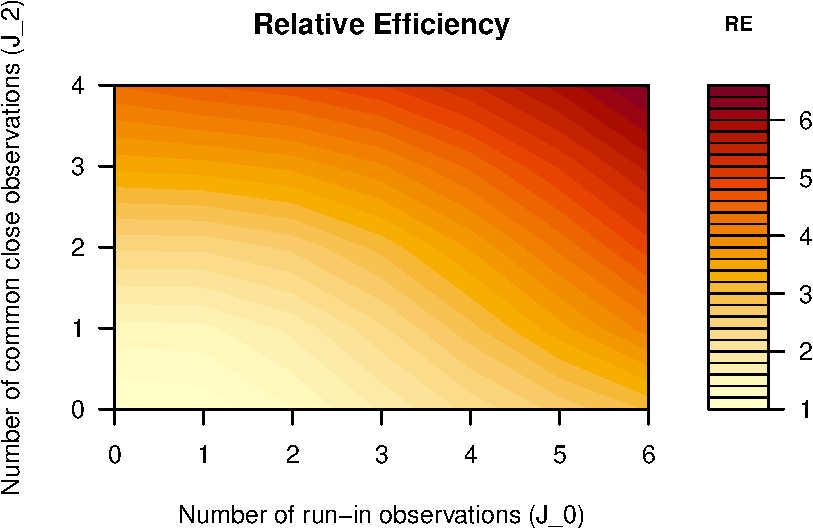
\includegraphics[keepaspectratio,alt={Relative efficiency of run-in and common close designs compared to the standard design (J\_0=0, J\_2=0) with the same number of post-randomization observations (J\_1=2). Parameters: \textbackslash sigma\^{}2 = 1, \textbackslash sigma\_b\^{}2 = 1, t = 1.}]{report_files/report_files/figure-latex/fig_efficiency-1.pdf}}
\caption{Relative efficiency of run-in and common close designs compared
to the standard design (\(J_0=0\), \(J_2=0\)) with the same number of
post-randomization observations (\(J_1=2\)). Parameters:
\(\sigma^2 = 1\), \(\sigma_b^2 = 1\), \(t = 1\).}
\end{figure}

\subsection{Application: Alzheimer's disease imaging
trial}\label{application-alzheimers-disease-imaging-trial}

Using variance parameters estimated from the MIRIAD dataset
(\citeproc{ref-frostOptimizingDesignClinical2008}{Frost et al. 2008}):
\(\sigma_b^2 = 0.9745\) (between-subject slope variance),
\(\sigma^2 = 0.0025\) (residual variance), with observation interval
\(t = 1\) year and treatment effect \(\Delta = 0.25\) (25\% reduction in
atrophy rate relative to placebo rate of approximately 1.0\% brain
volume loss per year).

\begin{longtable}[]{@{}rrrrr@{}}
\caption{Sample size per group for AD imaging trial (\(J_1=2\)
post-randomization visits, \(\Delta = 0.25\), 90\% power). Top 15
configurations by sample size.}\tabularnewline
\toprule\noalign{}
\(J_0\) & \(J_1\) & \(J_2\) & \(m\) per group & Total visits \\
\midrule\noalign{}
\endfirsthead
\toprule\noalign{}
\(J_0\) & \(J_1\) & \(J_2\) & \(m\) per group & Total visits \\
\midrule\noalign{}
\endhead
\bottomrule\noalign{}
\endlastfoot
3 & 2 & 0 & 1 & 6 \\
4 & 2 & 0 & 1 & 7 \\
2 & 2 & 1 & 1 & 6 \\
3 & 2 & 1 & 1 & 7 \\
4 & 2 & 1 & 1 & 8 \\
0 & 2 & 2 & 1 & 5 \\
1 & 2 & 2 & 1 & 6 \\
2 & 2 & 2 & 1 & 7 \\
3 & 2 & 2 & 1 & 8 \\
4 & 2 & 2 & 1 & 9 \\
2 & 2 & 0 & 2 & 5 \\
0 & 2 & 1 & 2 & 4 \\
1 & 2 & 1 & 2 & 5 \\
1 & 2 & 0 & 3 & 4 \\
\end{longtable}

\begin{verbatim}
## AD imaging trial sample sizes (per group):
\end{verbatim}

\begin{verbatim}
##   Standard (r=0, k=2, f=0): 329
\end{verbatim}

\begin{verbatim}
##   Run-in   (r=2, k=2, f=0): 2  (99% reduction)
\end{verbatim}

\begin{verbatim}
##   Full     (r=2, k=2, f=2): 1  (100% reduction)
\end{verbatim}

\section{Discussion}\label{discussion}

The results presented here formalize and extend the framework of Frost
et al. (\citeproc{ref-frostOptimizingDesignClinical2008}{2008}) by
providing explicit variance formulas for the treatment effect estimator
under designs that incorporate run-in and common close observations.
Three points merit discussion.

\textbf{When run-in observations are most beneficial.} The efficiency
gain from run-in observations depends on the ratio
\(\sigma_b^2 t^2 / \sigma^2\). When between-subject slope variability is
large relative to residual variance (as in neuroimaging outcomes), even
one or two run-in observations yield substantial sample size reductions.
For cognitive outcomes, where this ratio is typically less favorable,
the gains are more modest and the cost of extended study duration must
be weighed against the sample size reduction.

\textbf{Common close as a low-cost efficiency gain.} The common close
phase provides information about individual trajectories without
requiring participants to remain on treatment. Since treatment has
ceased, both groups contribute to estimation of the underlying slope
variability, effectively tightening the precision of the treatment
effect estimator. The marginal benefit of each additional common close
observation diminishes (as with run-in observations), but the first one
or two common close visits typically provide meaningful sample size
reductions, particularly when \(\sigma_b^2 t^2 / \sigma^2\) is large.

\textbf{Relationship to the two-period model.} The formulas derived here
are consistent with the two-period linear mixed effects model of Wang et
al. (\citeproc{ref-wangTwoPeriodLinear2019}{2019}). Their Scenario 1
(common slope across periods) corresponds to setting \(\delta = \beta\)
in our model, while their Scenario 2 (different slopes) corresponds to
the general case. The advantage of our formulation is the explicit
separation of run-in, treatment, and common close phases, enabling
direct optimization of the number of observations in each phase.

\textbf{Limitations.} The derivations assume equally spaced
observations, linear trajectories, and a random intercept plus random
slope covariance structure. Extensions to unequal spacing, nonlinear
progression, and more complex random effects structures (e.g., random
intercept-slope correlation) are possible within the same Woodbury
identity framework but yield more complex expressions that may not admit
simple closed forms. The formulas also assume no dropout; in practice,
the Dawson-Lagakos pattern-mixture approach
(\citeproc{ref-frostOptimizingDesignClinical2008}{Frost et al. 2008})
can be applied to adjust for anticipated attrition.

\section{Conflict of interest}\label{conflict-of-interest}

The author declares no conflicts of interest.

\section{Funding}\label{funding}

This work received no specific funding.

\section{Data availability statement}\label{data-availability-statement}

The \texttt{runinpower} R package, the four companion manuscripts of
this compendium, the MATLAB symbolic-derivation scripts, and the shared
bibliography are openly available in the project repository. Specific
paths are listed in the Reproducibility section below.

\section{Reproducibility}\label{reproducibility}

This manuscript was rendered with R 4.4.x. Principal packages used are
the in-package \texttt{runinpower} source (nine source files:
allocation, ancova, averaged, covariance, covariance-ar1, design, power,
replicated, variance), \texttt{tinytest} (testing harness), and
\texttt{rmarkdown} plus \texttt{bookdown} for the manuscript build.
MATLAB symbolic derivations supporting the Woodbury-based variance
formulas are at \texttt{analysis/scripts/}.

\textbf{Random-number generator.} The variance formulas are
deterministic given fixed input parameters; no RNG is exercised. Where
Monte Carlo benchmarking against the analytic formulas is reported, the
driver sets \texttt{set.seed(20260418)} at its entry point.

\textbf{Data and code availability.} The R package source is at
\texttt{R/}. MATLAB scripts are at \texttt{analysis/scripts/}. The
companion manuscripts are at \texttt{analysis/paper\{2,3,4\}-*/}. The
manuscript source and shared bibliography (\texttt{../references.bib})
are at \texttt{analysis/paper1-runin-power/}.

\section*{References}\label{references}
\addcontentsline{toc}{section}{References}

\protect\phantomsection\label{refs}
\begin{CSLReferences}{1}{1}
\bibitem[\citeproctext]{ref-ard2011}
Ard, M. Colin, and Steven D. Edland. 2011. {``Power Calculations for
Clinical Trials in {Alzheimer's} Disease.''} \emph{Journal of
Alzheimer's Disease} 21: 369--77.
\url{https://doi.org/10.3233/JAD-2011-0062}.

\bibitem[\citeproctext]{ref-diggle2002}
Diggle, Peter J., Patrick Heagerty, Kung-Yee Liang, and Scott L. Zeger.
2002. \emph{Analysis of Longitudinal Data}. 2nd ed. Oxford University
Press.

\bibitem[\citeproctext]{ref-frisonLinearlyDivergentTreatment1997}
Frison, Lars J., and Stuart J. Pocock. 1997. {``Linearly Divergent
Treatment Effects in Clinical Trials with Repeated Measures: Efficient
Analysis Using Summary Statistics.''} \emph{Statistics in Medicine} 16
(24): 2855--72.
\url{https://doi.org/10.1002/(SICI)1097-0258(19971230)16:24\%3C2855::AID-SIM749\%3E3.0.CO;2-Y}.

\bibitem[\citeproctext]{ref-frostOptimizingDesignClinical2008}
Frost, Chris, Michael G. Kenward, and Nick C. Fox. 2008. {``Optimizing
the Design of Clinical Trials Where the Outcome Is a Rate. {Can}
Estimating a Baseline Rate in a Run-in Period Increase Efficiency?:
{THE} {EFFICIENCY} {OF} {CLINICAL} {TRIALS} {WITH} {A} {RUN}-{IN}
{DESIGN}.''} \emph{Statistics in Medicine} 27 (19): 3717--31.
\url{https://doi.org/10.1002/sim.3280}.

\bibitem[\citeproctext]{ref-hu2021}
Hu, Na, Hugh Mackey, and Ronald G. Thomas. 2021. {``Power Formulas for
Mixed Effects Models with Random Slope and Intercept Comparing Rate of
Change Across Groups.''} \emph{International Journal of Biostatistics},
ahead of print. \url{https://doi.org/10.1515/ijb-2020-0107}.

\bibitem[\citeproctext]{ref-iddi2022}
Iddi, Samuel, and Michael C. Donohue. 2022. {``Power and Sample Size for
Longitudinal Models in {R} -- the Longpower Package and {Shiny} App.''}
\emph{The R Journal} 14 (1): 264--82.
\url{https://journal.r-project.org/articles/RJ-2022-022/}.

\bibitem[\citeproctext]{ref-lairdlRandomEffectsModelsLongitudinal2023}
Lairdl, Nan M, and James H Warel. 2023. \emph{Random-{Effects} {Models}
for {Longitudinal} {Data}}.

\bibitem[\citeproctext]{ref-liuliang1997}
Liu, Guanghan, and Kung-Yee Liang. 1997. {``Sample Size Calculations for
Studies with Correlated Observations.''} \emph{Biometrics} 53: 937--47.
\url{https://doi.org/10.2307/2533554}.

\bibitem[\citeproctext]{ref-lu2010}
Lu, Kaifeng. 2010. {``On Efficiency of Constrained Longitudinal Data
Analysis Versus Longitudinal Analysis of Covariance.''}
\emph{Biometrics} 66 (3): 891--96.
\url{https://doi.org/10.1111/j.1541-0420.2009.01322.x}.

\bibitem[\citeproctext]{ref-lu2009}
Lu, Kaifeng, Devan V. Mehrotra, and Guanghan Frank Liu. 2009. {``Sample
Size Determination for Constrained Longitudinal Data Analysis.''}
\emph{Statistics in Medicine} 28 (4): 679--99.
\url{https://doi.org/10.1002/sim.3507}.

\bibitem[\citeproctext]{ref-packerWhyHasRunIn2017}
Packer, Milton. 2017. {``Why {Has} a {Run}-{In} {Period} {Been} a
{Design} {Element} in {Most} {Landmark} {Clinical} {Trials}? {Analysis}
of the {Critical} {Role} of {Run}-{In} {Periods} in {Drug}
{Development}.''} \emph{Journal of Cardiac Failure} 23 (9): 697--99.
\url{https://doi.org/10.1016/j.cardfail.2017.07.401}.

\bibitem[\citeproctext]{ref-sperlingA4StudyStopping2014}
Sperling, Reisa A., Dorene M. Rentz, Keith A. Johnson, et al. 2014.
{``The {A4} {Study}: {Stopping} {AD} {Before} {Symptoms} {Begin}?''}
\emph{Science Translational Medicine} 6 (228): 228fs13--13.
\url{https://doi.org/10.1126/scitranslmed.3007941}.

\bibitem[\citeproctext]{ref-wangTwoPeriodLinear2019}
Wang, Guoqiao, Andrew J. Aschenbrenner, Yan Li, et al. 2019.
{``Two‐period Linear Mixed Effects Models to Analyze Clinical Trials
with Run‐in Data When the Primary Outcome Is Continuous: {Applications}
to {Alzheimer}'s Disease.''} \emph{Alzheimer's \& Dementia:
Translational Research \& Clinical Interventions} 5 (1): 450--57.
\url{https://doi.org/10.1016/j.trci.2019.07.007}.

\bibitem[\citeproctext]{ref-wangProportionalConstrainedLongitudinal2022}
Wang, Guoqiao, Lei Liu, Yan Li, et al. 2022. {``Proportional Constrained
Longitudinal Data Analysis Models for Clinical Trials in Sporadic
{Alzheimer}'s Disease.''} \emph{Alzheimer's \& Dementia: Translational
Research \& Clinical Interventions} 8 (1).
\url{https://doi.org/10.1002/trc2.12286}.

\bibitem[\citeproctext]{ref-Zhao2021}
Zhao, Yu, and Steven D. Edland. 2021. {``Power Formulas for Mixed
Effects Models with Random Slope and Intercept Comparing Rate of Change
Across Groups.''} \emph{International Journal of Biostatistics}, ahead
of print. \url{https://doi.org/10.1515/ijb-2020-0107}.

\end{CSLReferences}

\end{document}
